\documentclass[conference, doublecolumn]{IEEEtran}
\IEEEoverridecommandlockouts
\usepackage{cite}
\usepackage{amsmath,amssymb,amsfonts}
\usepackage{algorithmic}
\usepackage{graphicx}
\usepackage{textcomp}
\usepackage{xcolor}
\usepackage{flushend}
\usepackage{hyperref}

\begin{document}

\title{\textbf{SP 2023 IOT102 Attendance Check}\\}

\author{
1\textsuperscript{st} Nha Tran Kim, 2\textsuperscript{nd} Dat Viet Tran, 3\textsuperscript{rd} Tai Dang, 4\textsuperscript{th} Hoa Quang Luu, and Duc Ngoc Minh Dang\\
FPT University, Ho Chi Minh Campus, Vietnam\\
\{nhatkse182290, dattvse180348, dattvse180348, hoalqse183138\}@fpt.edu.vn, and ducdnm2@fe.edu.vn}
\maketitle

\begin{abstract}
This project presents the design and implementation of an attendance check system utilizing a Fingerprint Sensor AS608 XD-65 Module, a WiFi NodeMcu ESP8266 CH340, and an LCD 1602 display. The system leverages biometric authentication through the fingerprint sensor to accurately log attendance data. The WiFi-enabled NodeMCU ESP8266 serves as the core processing unit, managing communication between the fingerprint sensor and the LCD display while facilitating wireless data transmission to a remote server or cloud platform for storage and analysis. The LCD 1602 display provides real-time feedback to users regarding the authentication status. This project demonstrates the integration of cost-effective components to create an efficient and scalable attendance management solution suitable for educational institutions and organizations.
\end{abstract}

\section{\textbf{Introduction}}

Biometric Integration: Developing efficient methods for integrating biometric technologies, such as fingerprint recognition, into attendance management systems.\\
Cost-Effectiveness: Designing cost-effective solutions that utilize affordable components while ensuring performance and scalability.\\
Cloud-Based Solutions: Investigating cloud-based attendance management systems to leverage the benefits of remote access, scalability, and data analytics.



\section{\textbf{Main proposal}}

\subsection{System models and block diagram}
In this diagram, LCD 1602 Display, Buzzer, Red \& Green Leds will be connected to WiFi NodeMcu ESP8266. WiFi NodeMcu ESP8266 is responsible for processing the input signals from the Fingerprint sensor and managing user input through buttons or other input devices. The WiFi NodeMcu ESP8266 sends the processed signals to the display, which typically consists of a Liquid Crystal Display (LCD) to display the information. 
\begin{figure}[htbp]
\centering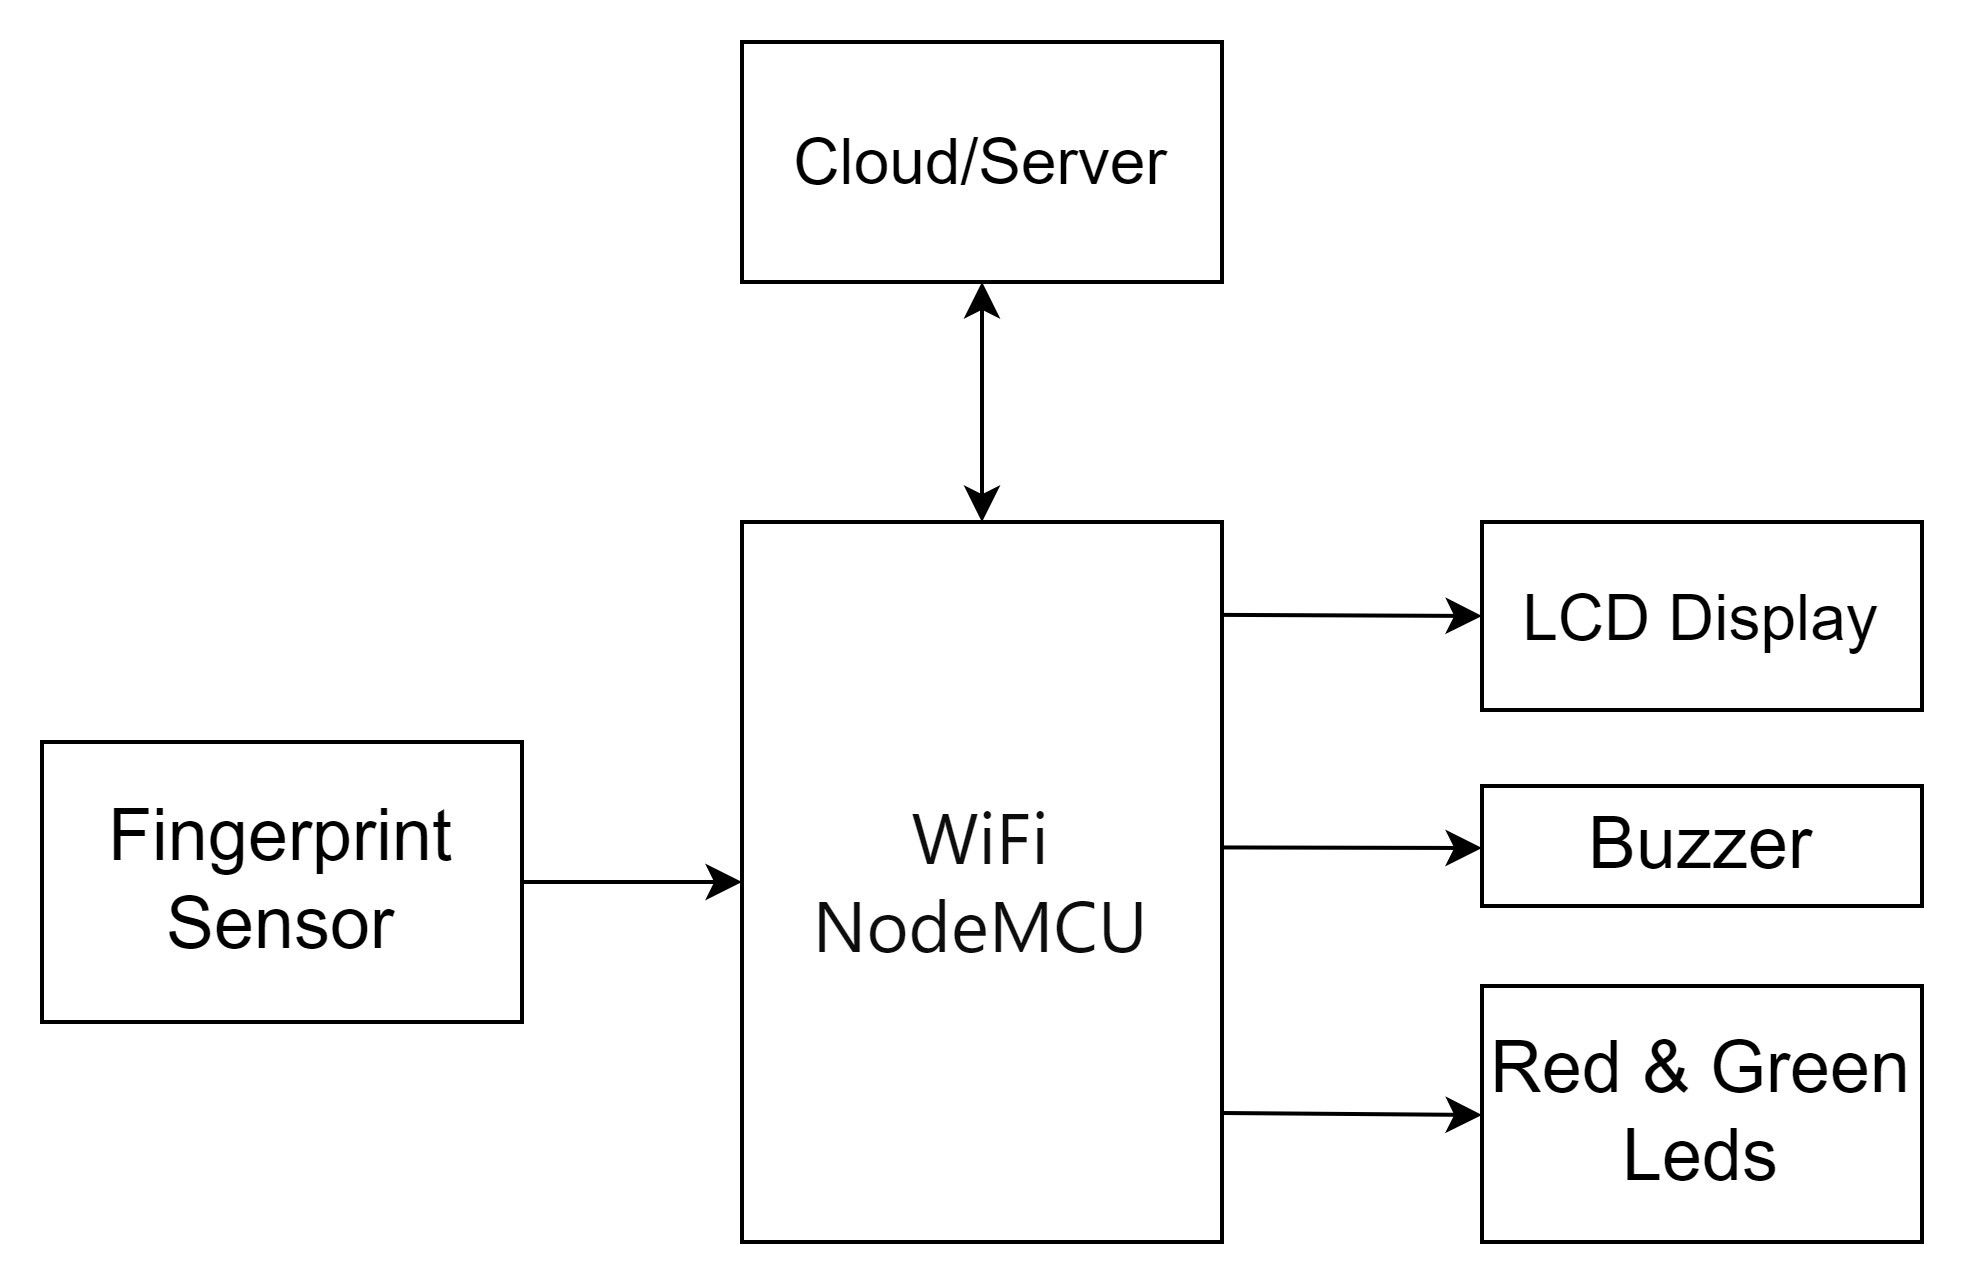
\includegraphics[width=2.6in]{block_diagram.jpg}
\caption{Block diagram of the developed system.}
\label{fig}
\end{figure}
\subsection{Components and peripheral devices}
\begin{table}[htbp]
\caption{SYSTEM’S COMPONENTS AND PERIPHERAL DEVICES}
\begin{center}
\begin{tabular}{|c|l|l|c|}
\hline
\textbf{No}&\textbf{Components/devices}  \\
\hline
1 & WiFi NodeMcu ESP8266 CH340  \\
\hline
2 & Fingerprint Sensor AS608 XD-65\\
\hline
3 & LCD 1602 Display \\
\hline
4 & Buzzer \\
\hline
5 & Red \& Green LEDs \\
\hline
\end{tabular}
\label{tab1}

\end{center}
\end{table}
\subsubsection{WiFi NodeMcu ESP8266 CH340}
The brain of the attendance system can be programmed to perform a variety of functions, such as receiving data from fingerprint sensor, displaying data on LCD, and uploading data to Cloud Server. 
\subsubsection{Fingerprint Sensor AS608 XD-65}It is used to scan finger and store data of finger, up to 127 different fingerprints.
\subsubsection{LCD 1602 Display}Show some information such as matched or not matched messages, id of fingerprint. It is energy-efficient and can display high-quality
 text and graphics.
\subsubsection{Buzzer}Make a sound when the fingerprint is matched, three sounds when the fingerprint is not matched.
\subsubsection{Red \& Green Leds}Green LED will ON if checked successfully. Otherwise, red LED will ON.

\subsection{Software programming}
Source code: \href{https://drive.google.com/drive/folders/1Zr50cyBe2i8WDqsiBBCLub8rHfnfoXOh?usp=drive_link}{here}
\subsection{Programming Flowchart}

\section{\textbf{Results and discussion}}

\subsection{Prototype Implementation}
Click \href{https://youtu.be/Myt8jY4ko3I}{here} to watch video.
\subsection{Experimental Results}

\subsection{Discussion}The attendance check system leveraging WiFi ESP8266 and a fingerprint sensor marks a significant leap in attendance management technology.\\
Meanwhile, the fingerprint sensor offers a secure and reliable method for individual identification, minimizing the risk of fraudulent attendance records.\\
Ensuring the system`s ease of use for administrators and users alike, along with implementing robust security measures to safeguard sensitive attendance data, remains paramount for its success and adoption.\\
Integration with cloud-based platforms could streamline data management and accessibility, while support for additional biometric authentication methods could offer greater flexibility.\\
Ultimately, this technology holds immense promise for revolutionizing attendance management across various industries, offering a sophisticated yet user-friendly solution to an age-old administrative task.

\section{\textbf{Conclusion}}
In conclusion, the attendance check system utilizing WiFi ESP8266 and a fingerprint sensor offers an efficient and secure solution for tracking attendance. Despite challenges like optimizing power usage and improving fingerprint recognition accuracy, the project demonstrates significant potential. Future enhancements could include integrating with cloud-based platforms for streamlined data management and expanding biometric authentication options. Overall, the system provides a cost-effective and scalable solution for attendance management in various settings.\cite{iotdesignpro}\cite{electroniclinic}



\bibliographystyle{unsrt}  %use this for IT
\bibliography{references}
\end{document}